\documentclass[12pt]{article}
\usepackage[margin=1in]{geometry}
\usepackage{natbib}
\usepackage{setspace}
\usepackage{url}
\usepackage{hyperref}
\usepackage{booktabs}
\usepackage{graphicx}
\usepackage{float}

\doublespacing

\title{Telepathy vs. Talk: Comparing Shared Representations and Explicit Communication in LLM Agents}
\author{Author Name(s)}
\date{}

\begin{document}

\maketitle

\begin{abstract}
We investigate two paradigms of multi-agent coordination using Large Language Models (LLMs): explicit communication via message passing and implicit coordination via shared representation. We populate a bandwidth-constrained, partially observable grid world ($R_{vis}=1$) with GPT-5-Mini agents tasked with navigating a linear bottleneck. We find that shared representation effectively solves the search problem, with global map sharing achieving a 100\% success rate compared to 40\% in the silent baseline ($p < 0.001$). However, this perfect environmental knowledge introduces a ``Coordination Paradox,'' where synchronized pathfinding leads to high collision rates (5.2 per run) compared to the baseline (0.0). Conversely, explicit communication strategies, whether structured or freeform, fail to provide a statistically significant improvement over their baseline ($p > 0.05$). Qualitative analysis of agent decision traces suggests that the 1-turn latency of message passing hampers coordination, though it remains an open question whether zero-latency protocols would resolve these friction points. We conclude that while shared state solves search, distinct conflict-resolution protocols are required to manage the traffic bottlenecks it creates.
\end{abstract}

\section{Introduction}

Large language models are increasingly deployed as collections of interacting agents rather than as isolated systems. Frameworks such as AutoGen and MetaGPT make it easy to instantiate role-specialized LLM agents that solve tasks by exchanging messages, while more recent systems like MegaAgent focus on scaling these patterns to hundreds of agents with hierarchical task decomposition and shared message pools \citep{wu2023autogen,hong2023metagpt,wang2024megaagent}. In these settings, ``communication'' is usually understood in the intuitive sense: agents send natural language or lightly structured messages to one another, and coordination emerges from the conversational protocol plus the underlying model's priors about teamwork.

In parallel, there is growing interest in using LLM agents as inhabitants of synthetic worlds. Social simulation work populates toy towns or social networks with dozens or thousands of LLM-driven characters and studies their interactions over time \citep{park2023generative}, while other projects treat LLMs as embodied controllers in games or virtual environments. The Abstraction and Reasoning Corpus (ARC-AGI) offers grid-based visual puzzles that probe pattern discovery and generalization, becoming a touchstone for evaluating reasoning in models that operate on JSON or textual encodings of small grids \citep{chollet2019measure,arcprize2025arcagi}. Similarly, embodied agents like Voyager in Minecraft showcase how a single LLM can drive long-horizon behavior in an environment surfaced entirely as text or abstract state \citep{wang2023voyager,robison2025claudepokemon}.

A third strand of research studies communication and coordination under stronger experimental control, mostly in the multi-agent reinforcement learning community. Classic work on differentiable communication architectures used small partially observable grid worlds to show how agents can learn when and what to broadcast. More recent approaches add language grounding and human interpretability, for example by training policies to imitate messages produced by LLM teammates \citep{li2024language}. These studies give careful control over reward and topology but typically operate with learned, opaque symbol channels rather than the natural language priors of off-the-shelf models.

At the systems level, there is growing interest in ``communication'' as sharing internal representations rather than messages. KV cache reuse and prefix caching can dramatically reduce prefill latency, and recent work extends this to multiple fine-tuned models by selectively recomputing only specific layers \citep{liu2025droidspeak}. In these systems, no natural language flows between agents; they coordinate indirectly by reusing a shared latent state. This notion of communication via shared representations is conceptually quite different from conversational protocols, yet it is arguably closer to how large model deployments scale in practice.

Our project sits at the intersection of these threads. We construct a small, fully controllable grid world rendered as an ASCII map and accompanying JSON, populated by identical LLM agents. Each agent perceives only its immediate surroundings ($R_{vis}=1$). The action space is minimal: move cardinal directions, stay, or use a communication channel. Because the grid can be scaled and the number of agents varied, we can tune task difficulty and collision pressure without changing the interface.

Within this environment, we instantiate two paradigms. In the first, communication is explicit message passing. Agents can send structured JSON packets or freeform natural language messages to teammates, delivered through the textual interface. In the second, communication is implicit via shared representations. Agents maintain internal maps that are either merged when within radio range or synchronized globally. This setup allows us to ask: when given explicit channels, do agents discover useful protocols? When given only a shared representation, do they exploit it? And how do these modes compare to having no communication at all?

\section{The LLMGrid Environment}

We utilize \texttt{LLMGrid}, a deterministic, discrete-time simulation engine. The environment topology is a $30 \times 10$ grid world generated via a recursive backtracking algorithm (Generation Seed 606). This specific layout, the ``Long Corridor,'' was selected for its high connectivity index combined with narrow chokepoints (1-2 cells wide) that mandate agent interaction to prevent blocking.

\subsection{Simulation Dynamics}
Five agents operate within the grid with a fixed turn budget ($T=100$). The simulation proceeds in synchronized turns where the engine solicits actions from all agents, resolves conflicts, and advances the state.

\begin{itemize}
    \item \textbf{Visibility ($R_{vis}=1$):} Agents operate under severe partial observability, perceiving only their own coordinate and the four immediate cardinal neighbors.
    \item \textbf{Movement \& Conflict:} Agents plan moves ($N, E, S, W$) or $STAY$. If multiple agents attempt to enter the same cell, or if two agents attempt to swap positions, the engine resolves this as a \texttt{BLOCK\_AGENT} outcome. No displacement occurs, and the turn is consumed.
    \item \textbf{Latency:} To model realistic processing and network constraints, explicit messages sent at turn $t$ are delivered to recipients at turn $t+1$.
\end{itemize}

\subsection{The Agent Interface}
To support the specific affordances of the two experimental branches, the agent context window is structured differently for each paradigm. In the Communication branch (Branch 1), agents receive a sensor-based representation suited for relative navigation. The prompt includes a $3 \times 3$ local view of the grid, a \texttt{goal\_sensor} providing a compass bearing (e.g., ``NE'') and signal strength, and a text log of recent messages. They possess no global coordinate map. In contrast, the Shared Representation branch (Branch 2) provides agents with a visual ASCII grid representing their internal memory. Unvisited cells are marked \texttt{X}, walls \texttt{\#}, and free space \texttt{.}. In the Global condition, this ASCII block is the data structure synchronized across agents; when Agent A discovers a wall at $(x,y)$, the \texttt{X} at that coordinate in Agent B's prompt is strictly replaced by \texttt{\#} in the next turn.

\begin{figure}[H]
    \centering
    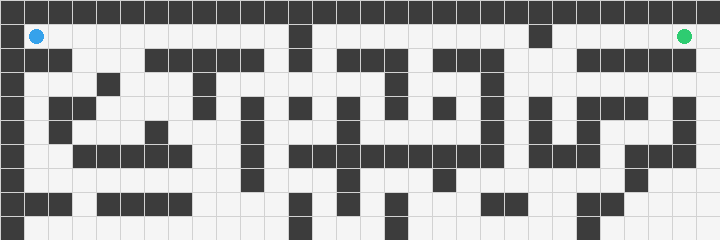
\includegraphics[width=0.8\textwidth]{figures/long_corridor_seed606.png}
    \caption{The ``Long Corridor'' Environment (Map Seed 606). The geometry remains constant across all experiments, while agent spawn locations vary by run seed.}
    \label{fig:grid}
\end{figure}

\begin{figure}[H]
    \centering
    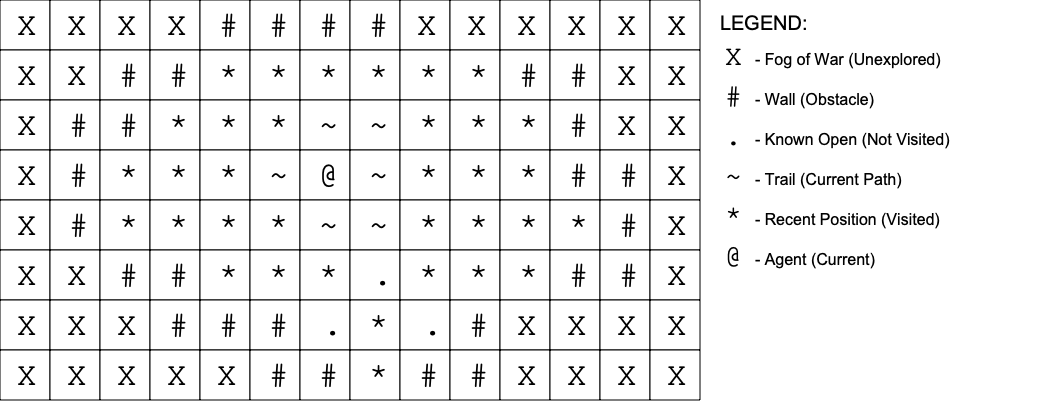
\includegraphics[width=0.7\textwidth]{figures/fog_of_war_example.png}
    \caption{Partial Observability (Fog of War). Agents perceive only their immediate neighborhood (visibility radius = 1). Gray cells represent unknown territory, demonstrating the exploration challenge agents face without shared representations.}
    \label{fig:interface}
\end{figure}

\section{Experimental Design}

We executed 90 total episodes. The variability in the experiment is controlled by two distinct random seeds and the sampling noise of the model.

\begin{itemize}
    \item \textbf{Map Seed (606):} Fixes the wall topology.
    \item \textbf{Run Seeds (13--17):} Five distinct integers used to initialize the pseudo-random number generator that places the 5 agents at start positions. These positions are randomized but guaranteed to be valid (non-wall) and equidistant from the goal relative to the grid difficulty.
    \item \textbf{Replicas ($N=3$):} For each Run Seed and Condition, we execute 3 independent runs. Since the engine is deterministic, variance between replicas is driven entirely by the non-deterministic sampling of the LLM.
\end{itemize}

We group the six conditions into two investigation branches. Each branch utilizes a specific control baseline matching its interface (Sensor vs. ASCII Map) to ensure fair comparison.

\begin{table}[H]
\centering
\caption{Unified Experimental Design Matrix ($N=15$ runs per condition)}
\label{tab:design}
\begin{tabular}{llccl}
\toprule
\textbf{Paradigm} & \textbf{Condition} & \textbf{Map Horizon} & \textbf{Comm.} & \textbf{Protocol / Constraints} \\
\midrule
\textit{Branch 1} & Baseline A & Local ($R=1$) & None & Silent control (Sensor Interface). \\
(Explicit) & Structured & Local ($R=1$) & $r=2$ & Schema: \texttt{INTENT} / \texttt{REQUEST}. \\
& Freeform & Local ($R=1$) & $r=2$ & Natural Language ($<96$ chars). \\
\midrule
\textit{Branch 2} & Baseline B & Local ($R=1$) & None & Silent control (ASCII Map Interface). \\
(Implicit) & Radio Sync & Radio ($r=2$) & None & Maps merge on contact. \\
& Global & Infinite & None & Oracle map shared instantly. \\
\bottomrule
\end{tabular}
\end{table}

All agents utilize the \texttt{azure:gpt-5-mini} model.

\subsection{Statistical Testing}
We use the Mann-Whitney U test (also called the Wilcoxon rank-sum test) to compare conditions. This non-parametric test is appropriate for our data because: (1) sample sizes are small ($N=15$ per condition), (2) we do not assume normal distributions, and (3) it is robust to outliers. The test statistic $U$ is computed by ranking all observations from both groups and summing the ranks for each group:
\begin{equation}
U = n_1 n_2 + \frac{n_1(n_1+1)}{2} - R_1
\end{equation}
where $n_1$ and $n_2$ are the sample sizes and $R_1$ is the sum of ranks for group 1. We report two-tailed p-values with significance threshold $\alpha = 0.05$.

\section{Results}

\subsection{Shared Representation Solves Search}
In the Map Sharing branch, the primary challenge is locating the goal. \textbf{Global Map Sharing} achieved a 100\% success rate (15/15 runs), compared to 40\% for the silent Baseline B and 60\% for Radio Sync.

Statistical analysis using the Mann-Whitney U test confirms this advantage is robust ($U=15.5$, $p < 0.001$). The shared representation effectively removes the search problem; agents immediately know the goal location and optimal path. Radio Sync provided a marginal improvement over the baseline, but the difference did not reach statistical significance ($p = 0.18$). This is largely explained by the ``Knowledge Plateau'': once agents dispersed beyond radio range ($r=2$), information propagation ceased, causing the discovery rate to flatline at approximately Turn 40.

\begin{figure}[H]
    \centering
    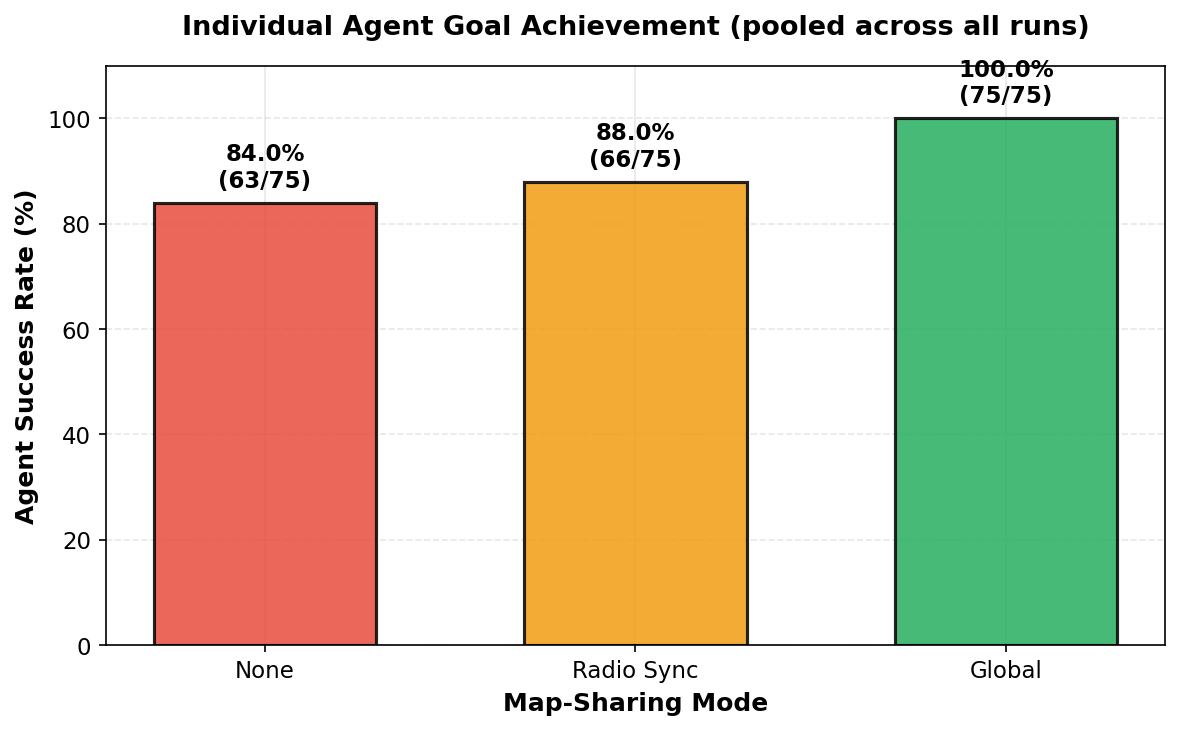
\includegraphics[width=0.8\textwidth]{figures/mapshare_agent_success_vs_baseline.png}
    \caption{Impact of Map Sharing on Task Completion. Global sharing guarantees success, while Radio synchronization fails to maintain connectivity sufficient to outperform the baseline significantly.}
    \label{fig:map_success}
\end{figure}

\subsection{Explicit Communication Fails to Coordinate}
In the Communication branch, agents must coordinate to move efficiently through the corridor. Neither \textbf{Structured} (56.0\% success) nor \textbf{Freeform} (62.7\% success) showed a statistically significant improvement over the silent Baseline A (57.3\%).

Comparison via Mann-Whitney U yielded $p=0.78$ for Freeform vs. Baseline and $p=0.84$ for Structured vs. Baseline. The hypothesis that explicit communication enables better coordination is not supported by the data in this bandwidth-constrained environment.

Furthermore, explicit communication failed to reduce collision rates. As shown in Figure \ref{fig:comm_collisions}, Freeform communication resulted in the highest average collision rate (20.9), compared to 19.7 for the Baseline and 16.3 for Structured. None of these differences were statistically significant ($p > 0.8$), indicating that the attempt to coordinate often introduced as much friction as it resolved.

\begin{figure}[H]
    \centering
    \begin{minipage}{0.48\textwidth}
        \centering
        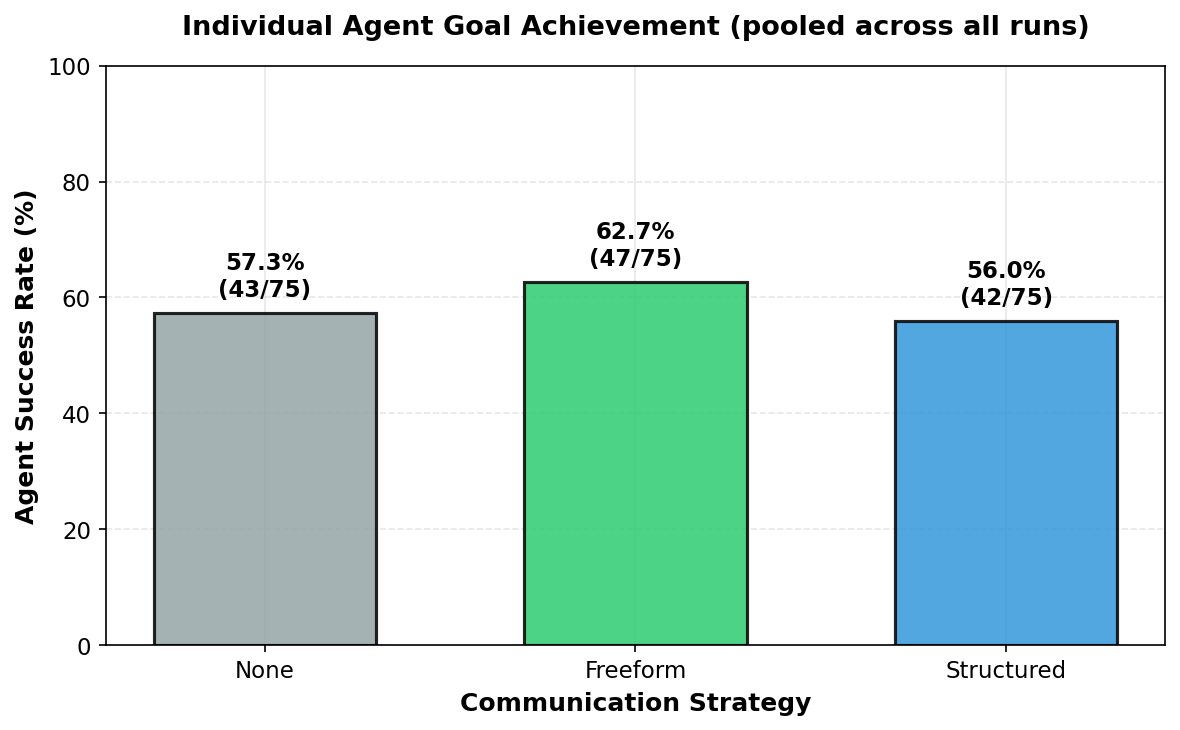
\includegraphics[width=\linewidth]{figures/communication_agent_success_vs_baseline.png}
    \end{minipage}
    \hfill
    \begin{minipage}{0.48\textwidth}
        \centering
        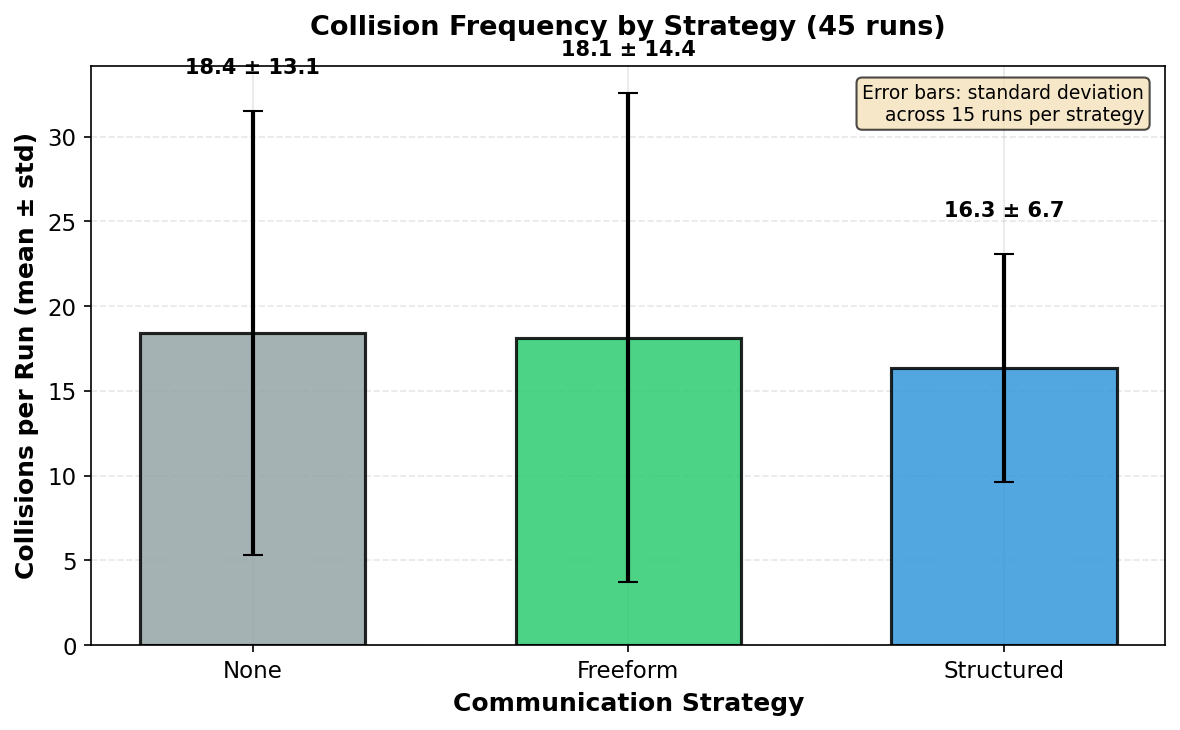
\includegraphics[width=\linewidth]{figures/communication_collision_rate_vs_baseline.png}
    \end{minipage}
    \caption{Inefficacy of Explicit Communication. Messaging strategies did not significantly improve success rates (Left) and failed to reduce collision rates compared to the silent baseline (Right).}
    \label{fig:comm_collisions}
\end{figure}

\begin{figure}[H]
    \centering
    % TODO: Add communication structure comparison image showing structured vs unstructured message examples
    % \includegraphics[width=0.8\textwidth]{figures/communication_structure_comparison.png}
    \caption{[PLACEHOLDER] Communication Structure Comparison. Examples of structured (INTENT/REQUEST schema) versus freeform natural language messages exchanged between agents.}
    \label{fig:comm_structure}
\end{figure}

\section{Discussion}

\subsection{The Coordination Paradox}
Global Map Sharing solved the search problem but introduced a distinct failure mode we term the ``Coordination Paradox.'' Agents in the Global condition experienced an average of \textbf{5.2 collisions per run} ($N=5$: [0, 2, 8, 0, 16]), compared to \textbf{0.0 collisions} in the Baseline B condition (all zeros). While this difference did not reach statistical significance with the available sample size ($p=0.072$, Mann-Whitney U), the observed pattern suggests that global knowledge may increase contention at bottlenecks. Further replication would be needed to confirm whether this trend represents a genuine tradeoff.

This paradox arises from independent optimization. Because all agents share the same oracle map, they calculate the exact same optimal path to the goal. In the logs for Seed 17, we observe agents separated by distance (outside $R_{vis}=1$) simultaneously identifying a bottleneck at $(10,1)$ as the optimal move. Without a mechanism to distinguish their roles or visualize one another, they converge on the cell at the same time, resulting in a \texttt{BLOCK\_AGENT} outcome. In the Baseline, agent ignorance acts as a noise filter, naturally distributing agents onto different sub-optimal paths and reducing contention.

\subsection{Phenomenological Analysis of Communication}
A detailed review of the turn-by-turn logs reveals why explicit communication failed to yield statistical gains, despite moments of apparent coordination.

\textbf{Structured Deadlocks:} In the Structured condition (Seed 15), we observe a ``Polite Deadlock.'' At Turn 21, Agent A broadcasts \texttt{INTENT: STAY} to yield. Due to the 1-turn latency, Agent B receives this at Turn 22. Wishing to reciprocate or clarify, Agent B broadcasts \texttt{INTENT: YIELD}. By the time Agent A receives this at Turn 23, the opportunity window has shifted, yet the agent often persists in signaling passivity. This cycle consumed 3 full turns of idleness, a high cost for a protocol intended to speed up navigation. The rigid schema allowed agents to declare state (``I am staying'') but struggled to support negotiation (``You go first'').

\textbf{Freeform Instruction:} The Freeform condition showed qualitatively richer interactions. In Seed 13, Agent A utilized the text field to send a complex instruction: \textit{"heading east to (10,1) next turn; please hold at (9,1)."} This differs fundamentally from the Structured intent; it is an instruction for the peer, not just a self-declaration. Agent B successfully parsed this, broadcast a confirmation, and held position. However, even this successful handshake required a ``stop-and-chat'' dynamic where agents paused to ensure safety. While phenomenologically impressive, the time cost of this caution neutralized the speed gains from collision avoidance, resulting in a success rate statistically indistinguishable from the silent baseline.

\section{Conclusion}

Our results indicate that in bandwidth-constrained environments, shared representations are a potent mechanism for multi-agent search, offering immediate performance gains over independent exploration. However, they do not inherently solve coordination; by aligning agent priors, they exacerbate contention in bottlenecks. Explicit communication, while theoretically capable of resolving this contention, appeared hampered by the realistic latency constraints ($T+1$) in our setup.

Future work should investigate whether eliminating the latency constraint (allowing synchronous, zero-shot communication blocks) would restore the efficacy of explicit protocols, or if better protocols can be designed that reduce collisions without imposing the high wait-costs observed here. Under the current constraints, we conclude that shared state effectively aligns context, but a distinct conflict-resolution mechanism is required to break the symmetry of optimal paths.

\bibliographystyle{plain}
\bibliography{refs}

\end{document}